\section{Distributed Memory}

\frame{\frametitle{Index}\tableofcontents[currentsection]}

\subsection{Partitioning}

\begin{frame}
	\frametitle{Distributed Memory: Mesh Partitioning}

	Mesh needs to be split between each processing unit.
	\begin{block}{Ideal partitioning method:}
		\begin{enumerate}
			\item Divide the mesh into $P$ partitions;
			\item Achieve good balance between partition sizes;
			\item Keep neighbourhood information;
			\item Minimize border between them, without compromising (2).
			\item Low partitioning overhead
		\end{enumerate}
	\end{block}

\end{frame}

\subsection{Implementation}

\begin{frame}
	\frametitle{Distributed Memory: Implementation}

	Division of the mesh based only on $x$ coordinate of cells:
	\begin{enumerate}
		\item Create ordered set of cells (key is $x$ coord)
		\item Sequentially assing $N/P$ cells to each process.
	\end{enumerate}

	\begin{multicols}{2}
		\begin{figure}
			\begin{center}
				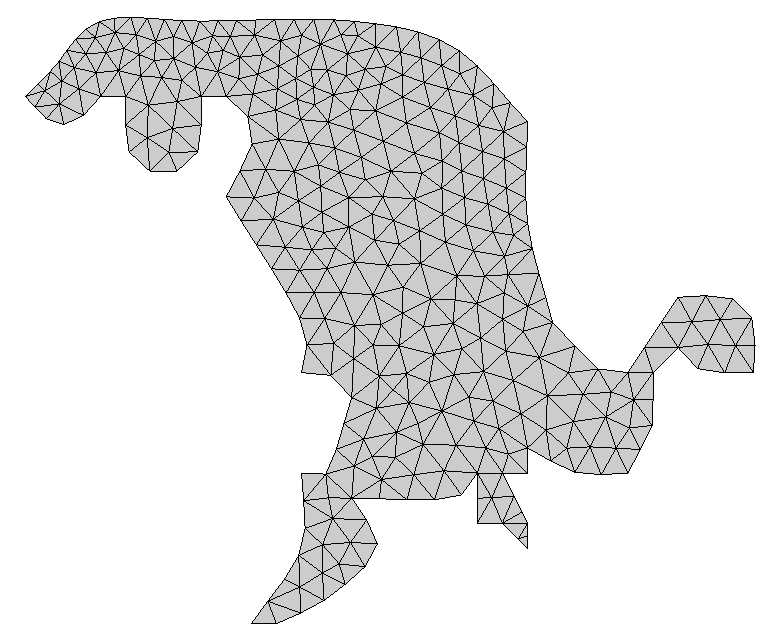
\includegraphics[width=0.955\columnwidth]{foz_msh}
			\end{center}
		\end{figure}
		\pause
		\begin{figure}
			\begin{center}
				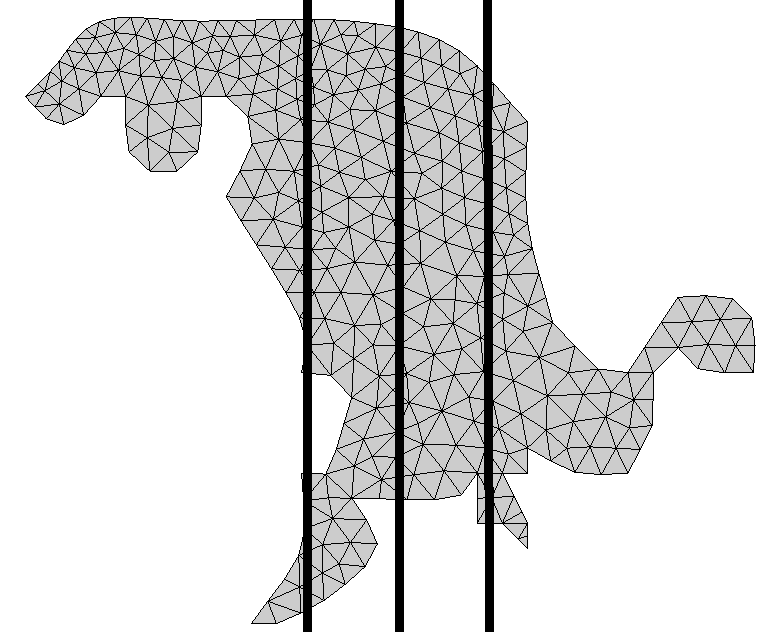
\includegraphics[width=0.955\columnwidth]{foz_p4_msh}
			\end{center}
		\end{figure}
	\end{multicols}
\end{frame}

\begin{frame}
	\frametitle{Distributed Memory: Implementation}

	\begin{block}{Two step communication}
		\begin{itemize}\itemsep=20pt
			\item Performed in two steps:
			\begin{enumerate}\itemsep=10pt
				\item Send to left / Receive from right
				\item Send to right / Receive from left
			\end{enumerate}

			\item Not homogeneous (no control over border size)

			\item Only 2 processes per node use the network
			\begin{itemize}
				\item Assuming best process asignement is used
			\end{itemize}
		\end{itemize}
	\end{block}
\end{frame}

\begin{frame}
\frametitle{Distributed Memory: Implementation}

	\begin{block}{Advantages}
		\begin{enumerate}\itemsep=10pt
			\item Simple concept and implementation
			\item Each partition has a left and a right neighbour
			\begin{itemize}
				\item[-] Communication in two steps only
			\end{itemize}
		\end{enumerate}
	\end{block}

	\begin{block}{Disadvantages}
		\begin{enumerate}\itemsep=10pt
			\item No control over size of border between partitions (communication)
			\item Sequential sort and distribution are slow
		\end{enumerate}
	\end{block}

\end{frame}

\begin{frame}
	\frametitle{Results}
	\begin{figure}
		\centering
		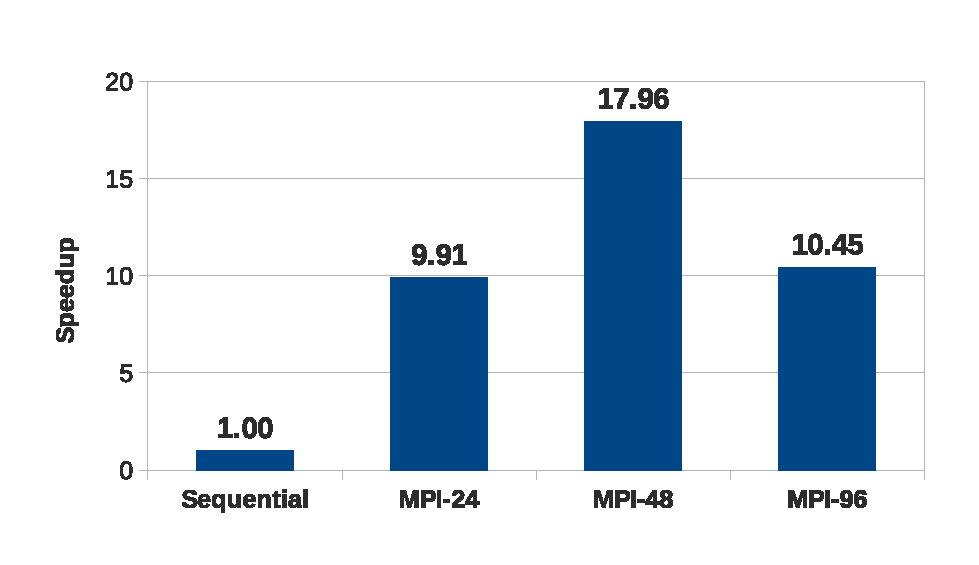
\includegraphics[width=0.8\textwidth]{graph_comparison_mpi.eps}
	\end{figure}
\end{frame}

